\subsection{Standard Signals}

\begin{figure}[h!]
\centering
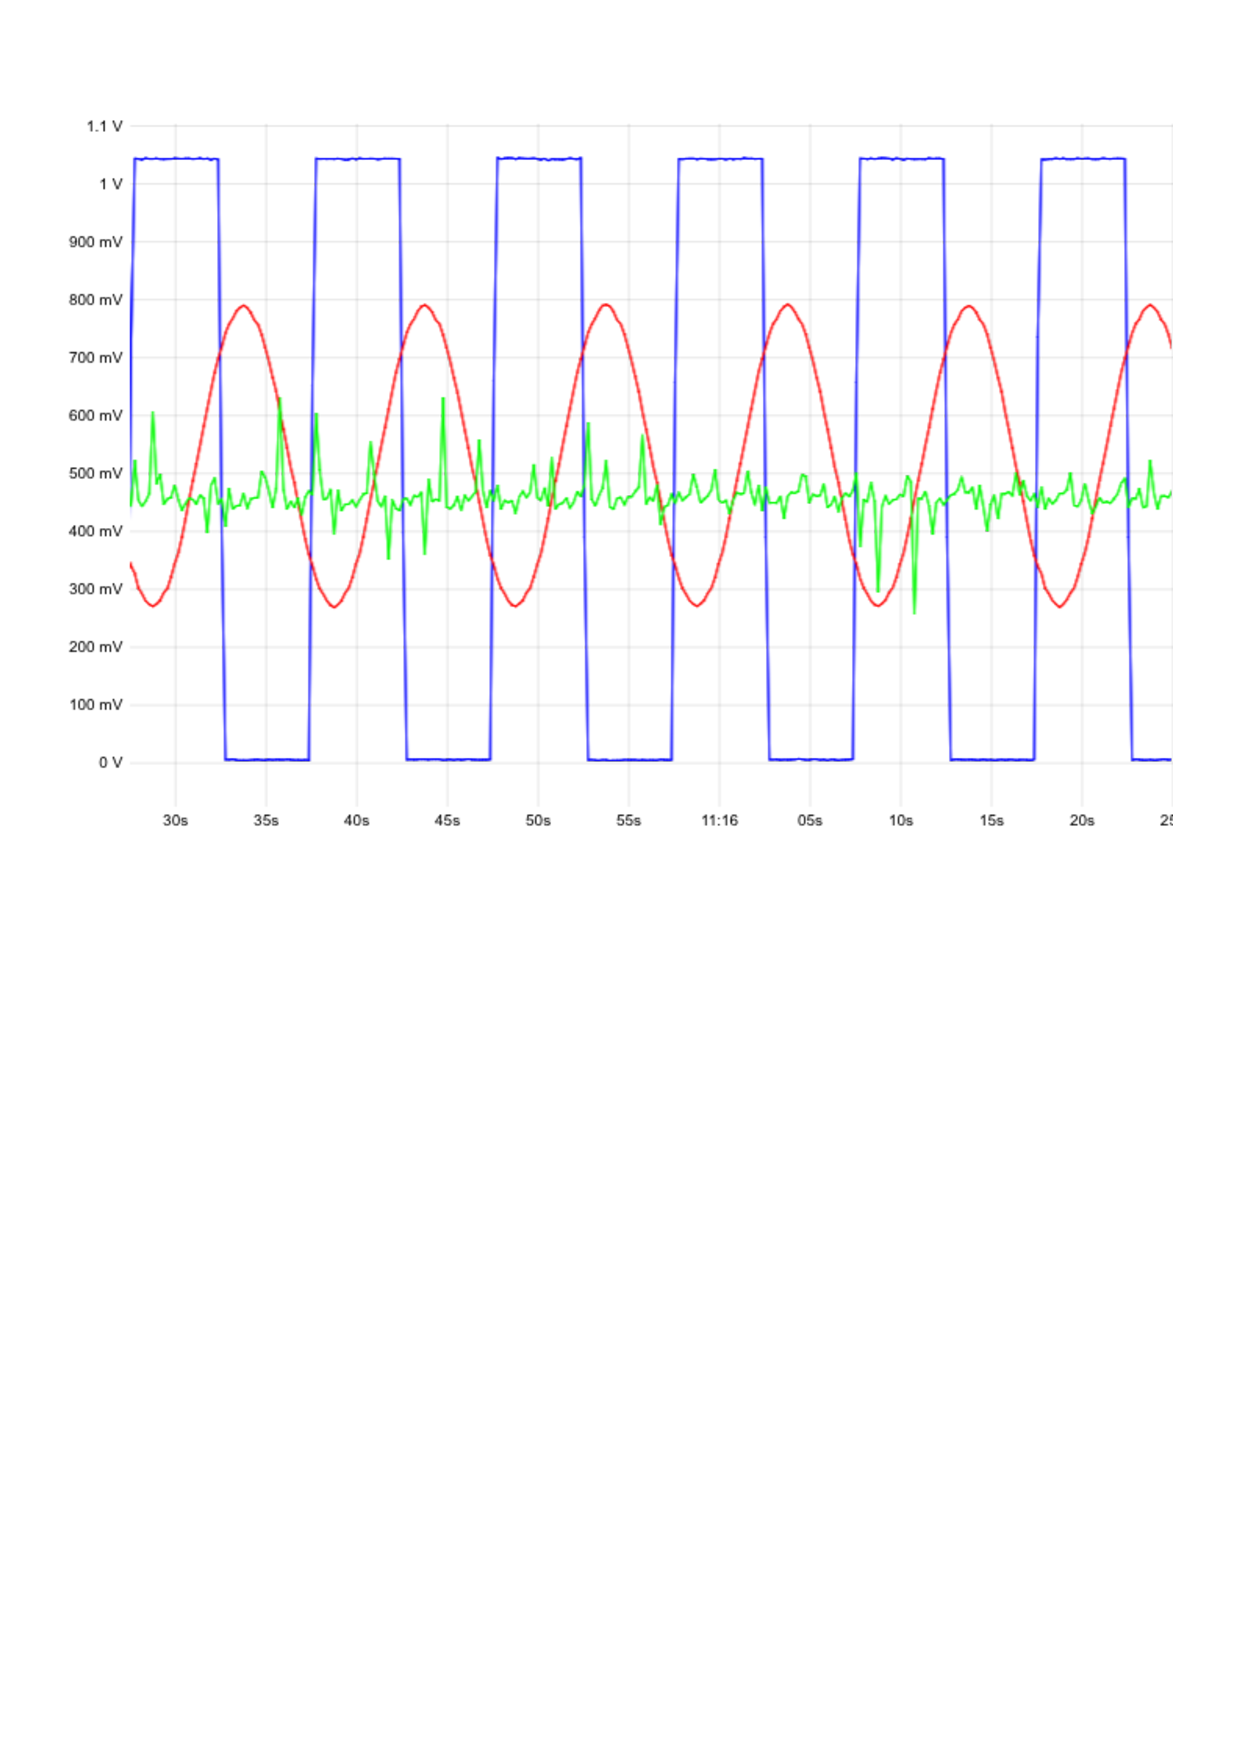
\includegraphics[trim={0cm 0cm 0cm  0cm}, clip, width=.75\textwidth]{./figures/standardsignals/picologChemComp.pdf}
\captionsetup{justification=centering}
\caption{Standard signals recorded using a PicoScope}
\label{fig: test1 picolog}
\bigbreak
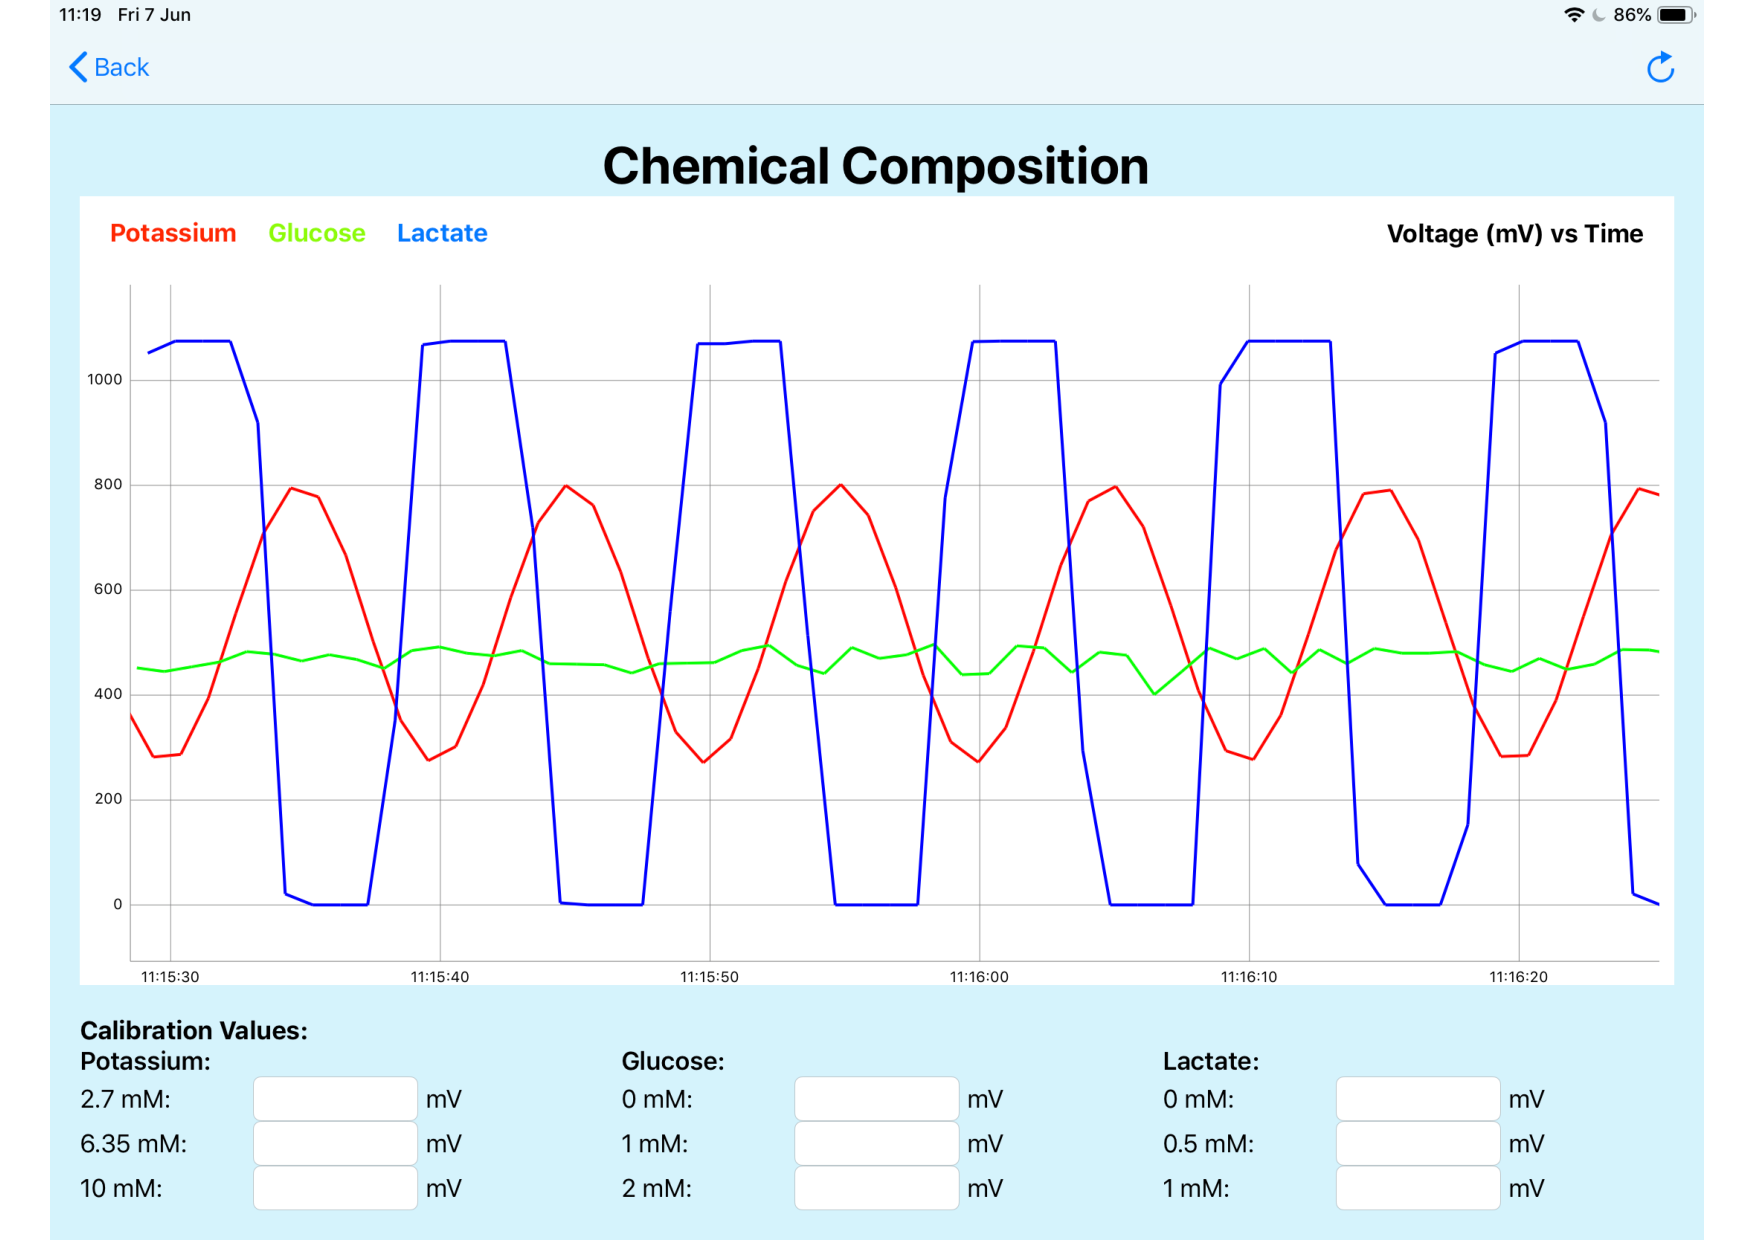
\includegraphics[trim={0cm 0cm 0cm  0cm}, clip, width=.75\textwidth]{./figures/standardsignals/appChemComp.pdf}
\captionsetup{justification=centering}
\caption{Standard signals recorded using the iPad app}
\label{fig: test1 app}
\end{figure}



Figure~\ref{fig: test1 picolog} shows the raw signals received on PicoLog, and Figure~\ref{fig: test1 app} shows the three signals received on the Chemical Composition page of the app after undergoing filtering and processing on the Arduino. The noise signal is shown in green in both plots, the square wave in blue, and the sine wave in red.


\subsection{Spreading Depolarisation}